\documentclass[border=10pt]{standalone}
\usepackage{tikz}
\usepackage{amsmath}
\usepackage{amssymb}
\usepackage{siunitx}
\usetikzlibrary{arrows.meta, calc, positioning}

\begin{document}
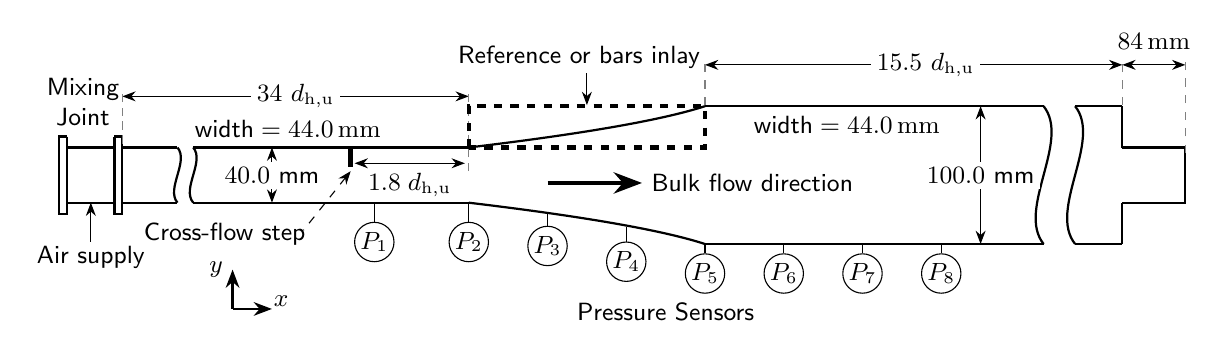
\begin{tikzpicture}[>=Stealth, every node/.style={font=\sffamily\small}]

    % Coordinate system
    \draw[thick, ->] (4.0,-1.7) -- (4.5,-1.7);
    \node[anchor=west] at (4.4, -1.6) {$x$};
    \draw[thick, ->] (4.0,-1.7) -- (4.0,-1.2);
    \node[anchor=east] at (4.0, -1.2) {$y$};

    % --- Left Section: Entry / Mixing Joint ---
    \draw[thick] (1.9, 0.49) -- (1.9, -0.49) -- (1.8, -0.49) -- (1.8, 0.49) -- (1.9, 0.49);

    \node[anchor=south, align=center] at (2.1, 0.5) {Mixing \\ Joint};

    \draw[thick] (1.9, 0.35) -- (2.5, 0.35);
    \draw[thick] (1.9, -0.35) -- (2.5, -0.35);
    \draw[thick] (2.5, 0.49) -- (2.5, -0.49) -- (2.6, -0.49) -- (2.6, 0.49) -- (2.5, 0.49);

    % Air supply annotation
    \draw[<-] (2.2, -0.35) -- (2.2, -0.85);
    \node[anchor=center, align=left] at (2.2, -1.05) {Air supply};

    % --- Main Tube Left (Narrow Section) ---
    \draw[thick] (2.6, 0.35) -- (3.3, 0.35);
    \draw[thick] (2.6, -0.35) -- (3.3, -0.35);

    % Vertical Wavy Break Lines at Inlet
    \draw[thick] (3.3, 0.35) .. controls (3.45, 0.175) and (3.15, -0.175) .. (3.3, -0.35);
    \draw[thick] (3.5, 0.35) .. controls (3.65, 0.175) and (3.35, -0.175) .. (3.5, -0.35);

    \draw[thick] (3.5, 0.35) -- (7.0, 0.35);
    \draw[thick] (3.5, -0.35) -- (7.0, -0.35);

    \node[anchor=south] at (4.7, 0.35) {$\text{width} = \qty{44.0}{\milli\metre}$};
    % \node[anchor=south] at (3.5, -0.85) {$\text{width} = \qty{44.0}{\milli\metre}$};

    % Cross-flow step
    \draw[ultra thick] (5.5, 0.35) -- (5.5, 0.1);
    \draw[<-, dashed] (5.5, 0.05) -- (4.9, -0.7);
    % \draw[dashed, gray] (7.0, 0.35) -- (7.0, 0.0);
    \node[anchor=east] at (5.05, -0.75) {Cross-flow step};
    \draw[<->] (5.55, 0.15) -- (6.95, 0.15);
    \node[anchor=north] at (6.25, 0.15) {$1.8\; d_\mathrm{h,u}$};
    

    % --- Central Section: Diffuser (curved walls) ---
    % Physical diffuser: x in [0, 195] mm, top wall y_top = 67.5 - sqrt(9025-40x)/2 mm.
    % This is the quadratic-formula solution of x = 9.5*(y-20) - (y-20)^2/10.
    % Scaling: x_mm = 65*(x_tikz-7)  [195 mm / 3 tikz units]
    %          y_tikz = 0.0175*y_mm   [0.35 tikz = 20 mm]
    % => y_tikz = 1.18125 - 0.00875*sqrt(9025 - 2600*(x_tikz-7))
    % Geometry is symmetric about y=0 (symmetry plane).
    \draw[thick] plot[domain=7.0:10.0, samples=60]
        (\x, {1.18125 - 0.00875*sqrt(9025 - 2600*(\x-7))});
    \draw[thick] plot[domain=7.0:10.0, samples=60]
        (\x, {-(1.18125 - 0.00875*sqrt(9025 - 2600*(\x-7)))});

    


    \draw[ultra thick, ->] (8.0, -0.1) -- (9.2, -0.1);
    \node[align=center, anchor=center] at (10.6, -0.1) {Bulk flow direction};

    % --- Main Tube Right (Wide Section) ---
    \draw[thick] (10.0, 0.875) -- (14.3, 0.875);
    \draw[thick] (10.0, -0.875) -- (14.3, -0.875);

    % Vertical Wavy Break Lines at Outlet
    \draw[thick] (14.3, 0.875) .. controls (14.65, 0.4375) and (13.95, -0.4375) .. (14.3, -0.875);
    \draw[thick] (14.7, 0.875) .. controls (15.05, 0.4375) and (14.35, -0.4375) .. (14.7, -0.875);

    \draw[thick] (14.7, 0.875) -- (15.3, 0.875);
    \draw[thick] (14.7, -0.875) -- (15.3, -0.875);

    % Outlet connection termination
    \draw[thick] (15.3, 0.875) -- (15.3, 0.35);
    \draw[thick] (15.3, -0.875) -- (15.3, -0.35);
    \draw[thick] (15.3, 0.35) -- (16.1, 0.35) -- (16.1, -0.35) -- (15.3, -0.35);

    \node[anchor=south] at (11.8, 0.4) {$\text{width} = \qty{44.0}{\milli\metre}$};

    % --- Dimensions and Annotations ---
    \draw[<->] (4.5, 0.35) -- (4.5, -0.35);
    \node[fill=white, inner sep=2pt] at (4.5, 0) {$40.0$ mm};

    \draw[<->] (13.5, 0.875) -- (13.5, -0.875);
    \node[fill=white, inner sep=2pt] at (13.5, 0) {$100.0$ mm};

    % Top Dimension L1
    \draw[<->] (2.6, 1.0) -- (7.0, 1.0);
    \node[fill=white, inner sep=2pt] at (4.8, 1.0) {$34\ d_\mathrm{h,u}$};
    \draw[densely dashed, gray] (2.6, 0.4) -- (2.6, 1.1);
    \draw[densely dashed, gray] (7.0, 0.05) -- (7.0, 1.1);

    % dashed box for inlay location
    \draw[ultra thick, dashed] (7.0, 0.35) -- (7.0, 0.875) -- (10.0, 0.875) -- (10.0, 0.35) -- (7.0, 0.35);
    \draw[<-] (8.5, 0.89) -- (8.5, 1.3);
    \node[anchor=center, align=center] at (8.4, 1.5) {Reference or bars inlay};

    % Top Dimension L2
    \draw[<->] (10.0, 1.4) -- (15.3, 1.4);
    \node[fill=white, inner sep=2pt] at (12.8, 1.4) {$15.5\ d_\mathrm{h,u}$};
    \draw[dashed, gray] (10.0, 0.885) -- (10.0, 1.5);
    \draw[dashed, gray] (15.3, 0.885) -- (15.3, 1.5);

    % Small outlet channel dimension
    \draw[<->] (15.3, 1.4) -- (16.1, 1.4);
    \node[fill=white, inner sep=2pt] at (15.7, 1.7) {\qty{84}{\milli\metre}};
    % \draw[dashed, gray] (10.0, 0.885) -- (10.0, 1.5);
    \draw[dashed, gray] (16.1, 0.28) -- (16.1, 1.5);

    % --- Pressure Sensors (P1 to P8) ---
    % P1, P2: inlet section, lower wall at y = -0.35
    \draw[solid] (5.8, -0.35) -- (5.8, -0.60); \draw (5.8, -0.85) circle (0.25) node {$P_1$};
    \draw[solid] (7.0, -0.35) -- (7.0, -0.60); \draw (7.0, -0.85) circle (0.25) node {$P_2$};

    % P3: diffuser entry, lower wall at x=7.8 (xi=0.8): y ~ -0.493
    \draw[solid] (8.0, -0.493) -- (8.0, -0.65); \draw (8.0, -0.90) circle (0.25) node {$P_3$};
    % P4: diffuser mid, lower wall at x=8.9 (xi=1.9): y ~ -0.686
    \draw[solid] (9.0, -0.66) -- (9.0, -0.85); \draw (9.0, -1.10) circle (0.25) node {$P_4$};

    % P5--P8: outlet section, lower wall at y = -0.875
    \draw[solid] (10.0, -0.875) -- (10.0, -0.99); \draw (10.0, -1.25) circle (0.25) node {$P_5$};
    \draw[solid] (11.0, -0.875) -- (11.0, -0.99); \draw (11.0, -1.25) circle (0.25) node {$P_6$};
    \draw[solid] (12.0, -0.875) -- (12.0, -0.99); \draw (12.0, -1.25) circle (0.25) node {$P_7$};
    \draw[solid] (13.0, -0.875) -- (13.0, -0.99); \draw (13.0, -1.25) circle (0.25) node {$P_8$};

    \node[anchor=north] at (9.5, -1.5) {\text{Pressure Sensors}};

\end{tikzpicture}
\end{document}
